\documentclass{beamer}
\usepackage[utf8]{inputenc}
\usepackage[ngerman]{babel}
\usepackage{url}
\usepackage{xcolor}
\usepackage{minted}
\usepackage[absolute,overlay]{textpos}

% Defines two commands:
% * \miniframesoff -- Disable the dots in the navigation bar
% * \miniframeson -- Enables the dots in the navigation bar
\makeatletter
\let\beamer@writeslidentry@miniframeson=\beamer@writeslidentry
\def\beamer@writeslidentry@miniframesoff{%
  \expandafter\beamer@ifempty\expandafter{\beamer@framestartpage}{}% does not happen normally
  {%else
    % removed \addtocontents commands
    \clearpage\beamer@notesactions%
  }
}
\newcommand*{\miniframeson}{\let\beamer@writeslidentry=\beamer@writeslidentry@miniframeson}
\newcommand*{\miniframesoff}{\let\beamer@writeslidentry=\beamer@writeslidentry@miniframesoff}
\makeatother
% Defines an environment for latexcode
\newenvironment{latexcode}
 {\VerbatimEnvironment
  \begin{VerbatimOut}{latexcode.out}}
  {\end{VerbatimOut}%
  \inputminted[breaksymbolindentleft=2,tabsize=4]{latex}{latexcode.out}}

\newenvironment{smalllatexcode}
 {\VerbatimEnvironment
  \begin{VerbatimOut}{latexcode.out}}
  {\end{VerbatimOut}%
  \inputminted[fontsize=\scriptsize]{latex}{latexcode.out}}
% Patch fancyvrb to support unicode
% It basically \detokenize everything before writing it to a file.
\makeatletter
\newcommand{\verbments@write@detok}[1]{%
  \immediate\write\FV@OutFile{\detokenize{#1}}}
\newcommand{\verbments@FVB@VerbatimOut}[1]{%
  \@bsphack
  \begingroup
  \FV@UseKeyValues
  \FV@DefineWhiteSpace
  \def\FV@Space{\space}%
  \FV@DefineTabOut
  \let\FV@ProcessLine\verbments@write@detok
  \immediate\openout\FV@OutFile #1\relax
  \let\FV@FontScanPrep\relax
  \let\@noligs\relax
  \FV@Scan}
\let\FVB@VerbatimOut\verbments@FVB@VerbatimOut
\makeatother

\usetheme[compress]{Berlin}
\setbeamerfont{headline}{size=\large}
\setbeamerfont*{section in head/foot}{size=\tiny}
\setbeamertemplate{toc}{circle}
\setbeamertemplate{itemize subitem}[triangle] % if you want a triangle
\setbeamercovered{transparent}

\definecolor{myBlue}{rgb}{0,0.55,0.8}
\usecolortheme[named=myBlue]{structure}

\newcommand{\slideheading}[1]{\textbf{#1}\\}

\title{Das \LaTeX-KBS}
\subtitle{\small Grundlagen von \LaTeX, Ti\textit{k}Z und Co.}
\author
{
	Walter Stieben \texttt{\href{mailto:4stieben@informatik.uni-hamburg.de}{4stieben@inf}}\\
	\href{http://hauke-stieler.de/}{Hauke Stieler} \texttt{\href{mailto:4stieler@informatik.uni-hamburg.de}{4stieler@inf}}
}
\date{\footnotesize 12.01.2016}

\begin{document}
	\maketitle
	\begin{frame}
		
	\end{frame}
		
	%%%%%%%%%%%%%%%%%%%%%%%%%%%%%%%%%%%%%%%%%%%%%%%%%%%%%%%%%%%%%%%%%%%%%%%
		
	\begin{frame}
		\begin{minipage}[t][0.5\textheight]{0.5\textwidth}
			\vspace{0pt} 
			\tableofcontents
		\end{minipage}
		\begin{minipage}[t]{0.45\textwidth} 
			\vspace{0pt}  
			
\includegraphics[width=\textwidth]{./images/gib-word-keine-chance}
		\end{minipage}
	\end{frame}
		
	%%%%%%%%%%%%%%%%%%%%%%%%%%%%%%%%%%%%%%%%%%%%%%%%%%%%%%%%%%%%%%%%%%%%%%%
		
	\section{Was ist \TeX{} und \LaTeX{}}
		\subsection*{}
		\begin{frame}{Was ist \LaTeX{}}
			\slideheading{\LaTeX{} und \TeX{}:}
			\begin{itemize}
				\item \TeX{} ist ein Textsatzsystem von Donald E. Knuth
				\item \LaTeX{} ist ein Satz von Makros für \TeX
				\item WYSIWYT (What You See Is What You Type)
			\end{itemize}
			\vspace{0.2cm}
			\slideheading{Vorteile von \LaTeX{}:}
			\begin{itemize}
				\item Ergebnis sieht hübsch aus
				\item \LaTeX{} kümmert sich um die Formatierung
				\item Der Quelltext lässt sich Versionsverwalten
				\item Für mathematische Formeln sehr gut
				\item ``Ich möchte X mit \LaTeX{} machen'' $\rightarrow$
				Suchmaschine: ``latex X'' eingeben $\rightarrow$
				Ergebnis in den Quelltext kopieren
			\end{itemize}
		\end{frame}
		
		%%%%%%%%%%%%%%%%%%%%%%%%%%%%%%%%%%%%%%%%%%%%%%%%%%%%%%%%%%%%%%%%%%%%%%%
		
		\begin{frame}{\LaTeX{} installieren}
			\slideheading{\LaTeX-Distribution:}
			\begin{description}
				\item[GNU/Linux] Nutzt den Paketmanager eurer Distribution. Debian/Ubuntu: \texttt{apt-get install texlive} 
				\item[Windows] MiKTeX herunterladen und installieren. \url{http://miktex.org/}
				\item[Mac OS] MacTex herunterladen und installieren. \url{http://tug.org/mactex/} 
			\end{description}
			\slideheading{\LaTeX-Editoren:}
			\begin{description}
				\item[Kile] Guter Editor für GNU/Linux (KDE).
				\item[Gummi] Editor für GNU/Linux (GTK) mit Live-Preview
				\item[AUCTeX] für Emacs-Benutzer
				\item[Texmaker] Editor für alle Betriebssysteme
			\end{description}
			 und viele mehr \dots
		\end{frame}
		
		%%%%%%%%%%%%%%%%%%%%%%%%%%%%%%%%%%%%%%%%%%%%%%%%%%%%%%%%%%%%%%%%%%%%%%%
		
		\begin{frame}{Verschiedene \LaTeX{}-Compiler}
			Es gibt verschiedenen Compiler für \LaTeX{}. Heute: \textbf{pdflatex}
			\vspace{0.2cm}
			\slideheading{Vorteile von pdflatex:}
			\begin{itemize}
				\item Direktes erzeugen einer PDF
				\item Viele PDF-Features nutzbar
				\item Einfach zu verwenden
			\end{itemize}
			\vspace{0.1cm}
			\slideheading{Nachteile von pdflatex:}
			\begin{itemize}
				\item Kein \texttt{pstricks} nutzbar.
				\item Postscript-Dateien nicht direkt einbindbar
				\item Keine vollständige Unicode-Unterstützung (wie Xe\LaTeX)
			\end{itemize}
		\end{frame}
		
		%%%%%%%%%%%%%%%%%%%%%%%%%%%%%%%%%%%%%%%%%%%%%%%%%%%%%%%%%%%%%%%%%%%%%%%
		
		\begin{frame}{Detexify -- \LaTeX-Symbolerkennung}
			\begin{center}
				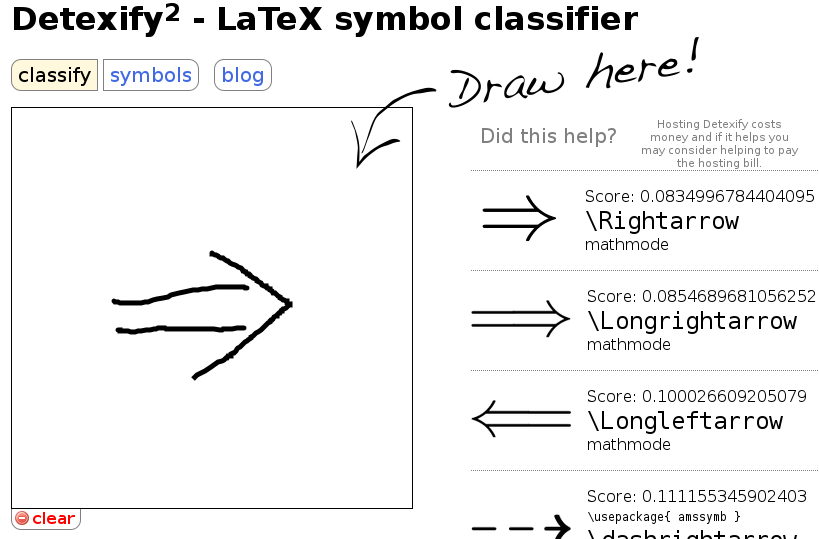
\includegraphics[width=0.95\textheight]{images/detexify}
				\vspace{0.3cm}
				
				\Large \href{http://detexify.kirelabs.org/}{http://detexify.kirelabs.org/}
			\end{center}
		\end{frame}
		
		%%%%%%%%%%%%%%%%%%%%%%%%%%%%%%%%%%%%%%%%%%%%%%%%%%%%%%%%%%%%%%%%%%%%%%%
		
		\begin{frame}{Anmerkungen}
			\slideheading{Achtung:} \TeX{} ist eine Programmiersprache! Lasst nur vertrauenswürdige
			Menschen \TeX/\LaTeX-Code auf eurem Rechner/Server ausführen.
			
			\vspace{0.2cm}
			\slideheading{Anmerkung:} Wenn du dir diese Folien anschaust, ist das System
			nicht mehr online. Es war nur zum Ausprobieren während des
			KunterBuntenSeminars gedacht.
		\end{frame}
		
		%%%%%%%%%%%%%%%%%%%%%%%%%%%%%%%%%%%%%%%%%%%%%%%%%%%%%%%%%%%%%%%%%%%%%%%
		
		\section{Theorie in \LaTeX{}}
		\subsection{Textsatz}
		
		\begin{frame}{Dokumentenklassen}
			\begin{itemize}
				\item Die Dokumentenklasse beschreibt wie ein Dokument aussieht
				\item Ihr beschreibt was ihr schreibt (z.\,B. was eine Überschrift ist)
				\item \LaTeX{} formatiert euer Dokument mit Hilfe der Dokumentenklasse, nicht ihr!
			\end{itemize}
			\vspace{0.2cm}
			Beispiele für Dokumentenklassen:
			\begin{description}
				\item[Scrartcl/article:] Artikel im Umfang von mehreren Seiten
				\item[Scrllr2/letter:] Briefe
				\item[Scrreprt/report:] Reports, Umfang mehr als 15 Seiten
				\item[Scrbook/book:] Bücher
			\end{description}
		\end{frame}
		
		%%%%%%%%%%%%%%%%%%%%%%%%%%%%%%%%%%%%%%%%%%%%%%%%%%%%%%%%%%%%%%%%%%%%%%%
		
		\begin{frame}{Syntax - Befehle und Umgebungen}
			\slideheading{Befehle:}
			\begin{itemize}
				\item Beginnen mit einem Backslash ( \textbackslash... )
				\item Parameter in geschweiften Klammern ( \{...\} )
				\item \textit{Optionale} Parameter in eckigen ( [...] )
				\item Manchmal auch als \texttt{*}-Variante (leicht verändertes Verhalten; s. \texttt{align} und \texttt{align*} Umgebung später)
			\end{itemize}
			\slideheading{Umgebungen:}
			\begin{itemize}
				\item Beginnen mit dem \texttt{\textbackslash begin\{name\}} Befehl
				\item und enden mit dem \texttt{\textbackslash end\{name\}} Befehl
				\item Formatieren ganze Textblöcke
			\end{itemize}
		\end{frame}
		
		%%%%%%%%%%%%%%%%%%%%%%%%%%%%%%%%%%%%%%%%%%%%%%%%%%%%%%%%%%%%%%%%%%%%%%%
		
		\begin{frame}{Aufbau des Dokumentes}
			\slideheading{Dokument:}
			\begin{enumerate}
				\item Dokumentenklasse wählen
				\item Pakete laden
				\item Einstellungen vornehmen, Styles ändern, Befehle definieren, et.
				\item Dokument öffnen
				\item Zeugs schreiben
				\item Dokument schließen
			\end{enumerate}
		\end{frame}
		
		%%%%%%%%%%%%%%%%%%%%%%%%%%%%%%%%%%%%%%%%%%%%%%%%%%%%%%%%%%%%%%%%%%%%%%%
		
		\section{Grundlagen mit \LaTeX{}}
		\subsection{Textsatz-Grundlagen}
		
		\begin{frame}[containsverbatim]{Mein erstes Dokument}
			\begin{latexcode}
\documentclass[a4paper,10pt]{scrartcl}
\usepackage[utf8]{inputenc}
\usepackage[T1]{fontenc}
\usepackage[ngerman]{babel}
\usepackage{lmodern}

\author{Max Mustermann}
\title{Mein erstes Dokument}

\begin{document}
	\maketitle{}
	Hello World!
\end{document}
			\end{latexcode}
			\begin{textblock}{10}(7.5,10.5)
				
\includegraphics[width=5.5cm]{images/erstes-dokument-scrartcl}
			\end{textblock}
		\end{frame}
		
		%%%%%%%%%%%%%%%%%%%%%%%%%%%%%%%%%%%%%%%%%%%%%%%%%%%%%%%%%%%%%%%%%%%%%%%
		
		\begin{frame}[containsverbatim]{Mein erstes Dokument}
			\begin{latexcode}
\documentclass[a4paper,10pt]{article}
\usepackage[utf8]{inputenc}
\usepackage[T1]{fontenc}
\usepackage[ngerman]{babel}
\usepackage{lmodern}

\author{Max Mustermann}
\title{Mein erstes Dokument}

\begin{document}
	\maketitle{}
	Hello World!
\end{document}
			\end{latexcode}
			\begin{textblock}{10}(7.5,10.5)
				
\includegraphics[width=5.5cm]{images/erstes-dokument-article}
			\end{textblock}
		\end{frame}
		
		%%%%%%%%%%%%%%%%%%%%%%%%%%%%%%%%%%%%%%%%%%%%%%%%%%%%%%%%%%%%%%%%%%%%%%%
		
		\begin{frame}[containsverbatim]{Gliederung des Dokumentes}
			\slideheading{\LaTeX-Code:}
			\begin{latexcode}
\section{Finden von maximalen Cliquen in Graphen}
Maximale Cliquen haben viele reale Anwendungsfälle.

\subsection{NP-Vollständigkeit}
Das Problem ist NP-vollständig.
			\end{latexcode}
			
			\vspace{0.1cm}
			\slideheading{Ergebnis:}
			\vspace{0.3cm}
			{\Large \textbf{1 Finden von maximalen Cliquen}}\\
			Maximale Cliquen haben viele reale Anwendungsfälle.\\
			\vspace{2mm}
			\textbf{1.1 NP-Vollständigkeit}\\
			Das Problem ist NP-vollständig.
		\end{frame}
		
		%%%%%%%%%%%%%%%%%%%%%%%%%%%%%%%%%%%%%%%%%%%%%%%%%%%%%%%%%%%%%%%%%%%%%%%
		
		\begin{frame}[containsverbatim]{Einfache Textformatierung}
			\slideheading{\LaTeX-Code:}
			\begin{latexcode}
Dieser Text besitzt einen\\
Zeilenumbruch.
Dieser Text\newline
auch

Dies ist ein Absatz
			\end{latexcode}
			
			\slideheading{Ergebnis:}
			\vspace{0.1cm}
			Dieser Text besitzt einen\\
			Zeilenumbruch
			Dieser Text\newline
			auch
			
			~~~~Dies ist ein Absatz
		\end{frame}
		
		%%%%%%%%%%%%%%%%%%%%%%%%%%%%%%%%%%%%%%%%%%%%%%%%%%%%%%%%%%%%%%%%%%%%%%%
		
		\begin{frame}[containsverbatim]{Einfache Textformatierung}
			\slideheading{\LaTeX-Code:}
			\begin{latexcode}
Dies ist \textbf{fett} oder \texttt{typewriter}
oder \textit{kursiv}. Oder einfach nur
\emph{hervorgehoben}.
			\end{latexcode}
			
			\slideheading{Ergebnis:}
			\vspace{0.1cm}
			Dies ist \textbf{fett} oder \texttt{typewriter} oder
			\textit{kursiv}. Oder einfach nur \emph{hervorgehoben}.
		\end{frame}
		
		%%%%%%%%%%%%%%%%%%%%%%%%%%%%%%%%%%%%%%%%%%%%%%%%%%%%%%%%%%%%%%%%%%%%%%%
		
		\begin{frame}[containsverbatim]{(Nummerierte) Auflistungen}
			\begin{columns}
				\column{.5\textwidth}
				\slideheading{\LaTeX-Code:}
				\begin{latexcode}
\begin{itemize}
	\item Kartoffeln
	\item Butter
	\item Milch
\end{itemize}
				\end{latexcode}
				
				\slideheading{Ergebnis:}
				\begin{itemize}
					\item Kartoffeln
					\item Butter
					\item Milch
				\end{itemize}
				 
				\column{.5\textwidth}
				\slideheading{\LaTeX-Code:}
				\begin{latexcode}
\begin{enumerate}
	\item Kartoffeln
	\item Butter
	\item Milch
\end{enumerate}
				\end{latexcode}
				
				\slideheading{Ergebnis:}
				\begin{enumerate}
					\item Kartoffeln
					\item Butter
					\item Milch
				\end{enumerate}
			\end{columns}
		\end{frame}
		
		%%%%%%%%%%%%%%%%%%%%%%%%%%%%%%%%%%%%%%%%%%%%%%%%%%%%%%%%%%%%%%%%%%%%%%%
		
		\begin{frame}[t,containsverbatim]{(Nummerierte) Auflistungen}
			\begin{columns}[t]
				\column{.5\textwidth}
				\slideheading{\LaTeX-Code:}
				\begin{latexcode}
\begin{itemize}
	\item Kartoffeln
	\begin{itemize}
		\item Festkochend
		\item Mehligkochend
	\end{itemize}
	\item Butter
	\item Milch
\end{itemize}
				\end{latexcode}
				\column{.5\textwidth}
				\slideheading{Ergebnis:}
				\begin{itemize}
					\item Kartoffeln
					\begin{itemize}
						\item Festkochend
						\item Mehligkochend
					\end{itemize}
					\item Butter
					\item Milch
				\end{itemize}
			\end{columns}
		\end{frame}
		
		%%%%%%%%%%%%%%%%%%%%%%%%%%%%%%%%%%%%%%%%%%%%%%%%%%%%%%%%%%%%%%%%%%%%%%%
		
		\begin{frame}[containsverbatim]{Definitionslisten}
			\slideheading{\LaTeX-Code:}
			\begin{latexcode}
\begin{description}
	\item[Kile] Guter Editor für GNU/Linux (KDE).
	\item[AUCTeX] für Emacs-Benutzer
	\item[Texmaker] Editor für alle Betriebssysteme
\end{description}
			\end{latexcode}
			
			\slideheading{Ergebnis:}
			\begin{description}
				\item[Kile] Einfacher Editor für GNU/Linux (KDE).
				\item[AUCTeX] für Emacs-Benutzer
				\item[Texmaker] Editor für alle Betriebssysteme
			\end{description}
		\end{frame}
		
		%%%%%%%%%%%%%%%%%%%%%%%%%%%%%%%%%%%%%%%%%%%%%%%%%%%%%%%%%%%%%%%%%%%%%%%
		
		\begin{frame}[containsverbatim]{Tabellen}
			\begin{columns}[t]
				\column{0.55\textwidth}
				\slideheading{\LaTeX-Code:}
				\begin{latexcode}
\begin{tabular}{l||c|r}
	Händler & Produkt & Preis\\
	\hline
	\hline
	Ohbi & Fliesen & 17,95\\
	Porsche & Motor & 270,15\\
	\hline
	Farber & Stift & 2,99
\end{tabular}
				\end{latexcode}
				
				\column{0.45\textwidth}
				\slideheading{Ergebnis:}
				\vspace{0.1cm}
				\begin{tabular}{l||c|r}
					Händler & Produkt & Preis\\
					\hline
					\hline
					Ohbi & Fliesen & 17,95\\
					Porsche & Motor & 270,15\\
					\hline
					Farber & Stift & 2,99
				\end{tabular}
			\end{columns}
		\end{frame}
		
		%%%%%%%%%%%%%%%%%%%%%%%%%%%%%%%%%%%%%%%%%%%%%%%%%%%%%%%%%%%%%%%%%%%%%%%
		
		\begin{frame}{Probleme mit Tabellen}
			\begin{itemize}
			\item \LaTeX{} handhabt \texttt{tabular} als Buchstaben
			\item Kein automatischer Umbruch bei Seitenumbruch. Keine Tabelle länger als eine Seite.
			\item Bei \texttt{l/r/c} keine automatische Spaltenbereite
			\end{itemize}
			
			\vspace{0.2cm}
			\slideheading{Effekt:}
			\begin{tabular}{l|l}
				Spalte 1 & Spalte 2 \\
				\hline
				Foo & Lorem ipsum dolor sit amet, consectetur adipiscing elit. Donec sit amet nunc condimentum augue hendrerit rutrum. \\
				Bar & Lorem ipsum dolor sit amet, consectetur adipiscing elit. Donec sit amet nunc condimentum augue hendrerit rutrum.
			\end{tabular}
		\end{frame}
		
		%%%%%%%%%%%%%%%%%%%%%%%%%%%%%%%%%%%%%%%%%%%%%%%%%%%%%%%%%%%%%%%%%%%%%%%
		
		\begin{frame}[containsverbatim]{Tabellen mit \texttt{longtable}}
			\slideheading{\LaTeX-Code:}
			\begin{latexcode}
\begin{tabular}{l|p{8cm}}
Spalte 1 & Spalte 2 \\
\hline
Foo & Lorem ipsum dolor sit amet [...] \\
Bar & Lorem ipsum [...]
\end{tabular}
			\end{latexcode}
			
			\slideheading{Ergebnis:}
			\begin{tabular}{l|p{8cm}}
				Spalte 1 & Spalte 2 \\
				\hline
				Foo & Lorem ipsum dolor sit amet, consectetur adipiscing elit. Donec sit amet nunc condimentum augue hendrerit rutrum. \\
				Bar & Lorem ipsum [...]
			\end{tabular}
		\end{frame}
		
		%%%%%%%%%%%%%%%%%%%%%%%%%%%%%%%%%%%%%%%%%%%%%%%%%%%%%%%%%%%%%%%%%%%%%%%
		
		\begin{frame}[containsverbatim]{Grafiken einbinden}
			\slideheading{\LaTeX-Code:}
			\begin{latexcode}
\usepackage{graphicx}

\includegraphics[width=3cm]{images/gnu}
			\end{latexcode}
			
			\slideheading{Ergebnis:}
			
\includegraphics[width=2.5cm]{images/gnu}
		\end{frame}
		
		%%%%%%%%%%%%%%%%%%%%%%%%%%%%%%%%%%%%%%%%%%%%%%%%%%%%%%%%%%%%%%%%%%%%%%%
		
		\begin{frame}[containsverbatim]{\texttt{ams}-Pakete der American Mathematical Society}
			Für komplexere mathematische Darstellungen müssen die
			\texttt{ams}-Pakete der American Mathematical Society eingebunden
			werden.
			
			\vspace{0.5cm}
			\slideheading{\LaTeX{}-Code:}
			\begin{latexcode}
%% Im Header
\usepackage{amsmath}
\usepackage{amsfonts}
\usepackage{amssymb}
			\end{latexcode}
		\end{frame}
		
		%%%%%%%%%%%%%%%%%%%%%%%%%%%%%%%%%%%%%%%%%%%%%%%%%%%%%%%%%%%%%%%%%%%%%%%
		
		\subsection{Mathematischer Textsatz}
		\begin{frame}[containsverbatim]{Mathe-Umgebung}
			Es gibt verschiedene Mathe-Umgebungen:
			\begin{itemize}
				\item Die \texttt{\$...\$} Umgebung
				\begin{itemize}
					\item Mathe innerhalb von Text (stammt nicht aus \LaTeX, sondern aus \TeX)
				\end{itemize}
				\item Die \texttt{\textbackslash(...\textbackslash)} Umgebung
				\begin{itemize}
					\item Mathe innerhalb von Text (stammt aus \LaTeX und funktioniert besser mit den Mathe-Paketen)
				\end{itemize}
				\item Die \texttt{\textbackslash[...\textbackslash]} Umgebung
				\begin{itemize}
					\item Einzeilige Matheumgebung für eine Formel/Gleichung
				\end{itemize}
			\end{itemize}
		\end{frame}
		
		%%%%%%%%%%%%%%%%%%%%%%%%%%%%%%%%%%%%%%%%%%%%%%%%%%%%%%%%%%%%%%%%%%%%%%%
		
		\subsection{Mathematischer Textsatz}
		\begin{frame}[containsverbatim]{Mathe-Umgebung}
			\slideheading{\LaTeX{}-Code:}
			\begin{latexcode}
Wir können im Text Wurzeln, wie z.\,B. \( \sqrt{2} \)
verwenden. Oder auch Matheformeln als ganzen Block:
\[ \sum_{k=1}^n k = \frac{n(n+1)}{2} \]
			\end{latexcode}
			
			\slideheading{Ergebnis:}
			Wir können im Text Wurzeln, wie z.\,B. \( \sqrt{2} \)
			verwenden. Oder auch Matheformeln als ganzen Block:
			\[ \sum_{k=1}^n k = \frac{n(n+1)}{2} \]
			
			\vspace{0.1cm}
			%% Rule fügt eine horizontale Linie ein. Diese ist so breit wie die 
			%% maximale Textbreite (\textwidth) und 0.3mm dick.
			\rule{\textwidth}{.3mm}
			\scriptsize{\slideheading{Merke:}
			Das \$-Symbol für Mathemodus ist aus \TeX{} und nicht aus \LaTeX{}. Die \LaTeX{}-Variante geht besser mit \texttt{ams}-Macros und Fehlern um.\vfill}
		\end{frame}
		
		%%%%%%%%%%%%%%%%%%%%%%%%%%%%%%%%%%%%%%%%%%%%%%%%%%%%%%%%%%%%%%%%%%%%%%%
		
		\subsection{Mathematischer Textsatz}
		\begin{frame}[containsverbatim]{Mathe-Umgebung}
			\slideheading{\LaTeX{}-Code:}
			\begin{latexcode}
Neben Summen ($\sum$) gibt es auch Integrale:
\[ \int_a^b f(x) \mathrm{d}x \]
			\end{latexcode}
			
			\slideheading{Ergebnis:}
			Neben Summen ($\sum$) gibt es auch Integrale:
			\[ \int_a^b f(x) \mathrm{d}x \]
		\end{frame}
		
		%%%%%%%%%%%%%%%%%%%%%%%%%%%%%%%%%%%%%%%%%%%%%%%%%%%%%%%%%%%%%%%%%%%%%%%
		
		\subsection{Mathematischer Textsatz}
		\begin{frame}[containsverbatim]{Mathe-Umgebung}
			\slideheading{\LaTeX{}-Code:}
			\begin{latexcode}
Die Probleminstanz \(\mathfrak{B}\) sei gegeben Durch
die Menge \(\mathbb{N}\) und einer Zahl \(n\), sowie
der Eingabe \(\mathcal{A}\).
			\end{latexcode}
			
			\slideheading{Ergebnis:}
Die Probleminstanz \(\mathfrak{B}\) sei gegeben Durch die Menge \(\mathbb{N}\) und einer Zahl \(n\), sowie der Eingabe \(\mathcal{A}\).
		\end{frame}
		
		%%%%%%%%%%%%%%%%%%%%%%%%%%%%%%%%%%%%%%%%%%%%%%%%%%%%%%%%%%%%%%%%%%%%%%%
		
		\begin{frame}[containsverbatim]{Mathebeispiele: Matrizen}
			\slideheading{\LaTeX{}-Code:}
			\begin{latexcode}
\begin{pmatrix}
	\cos(\alpha)  & \sin(\alpha) & 0 & 0 \\
	-\sin(\alpha) & \cos(\alpha) & 0 & 0 \\
	            0 &            0 & 1 & 0 \\
	            0 &            0 & 0 & 1
\end{pmatrix}
			\end{latexcode}
			
			\slideheading{Ergebnis:}
			\[
				\begin{pmatrix}
				\cos(\alpha)  & \sin(\alpha) & 0 & 0 \\
				-\sin(\alpha) & \cos(\alpha) & 0 & 0 \\
				            0 &            0 & 1 & 0 \\
				            0 &            0 & 0 & 1
				\end{pmatrix}
			\]
		\end{frame}
		
		%%%%%%%%%%%%%%%%%%%%%%%%%%%%%%%%%%%%%%%%%%%%%%%%%%%%%%%%%%%%%%%%%%%%%%%
		
		\begin{frame}[containsverbatim]{Mathebeispiele: Matrizen}
			\slideheading{\LaTeX{}-Code:}
			\begin{latexcode}
\begin{bmatrix}
	\cos(\alpha)  & \sin(\alpha) & 0 & 0 \\
	-\sin(\alpha) & \cos(\alpha) & 0 & 0 \\
	            0 &            0 & 1 & 0 \\
	            0 &            0 & 0 & 1
\end{bmatrix}
			\end{latexcode}
			
			\slideheading{Ergebnis:}
			\[
				\begin{bmatrix}
				\cos(\alpha)  & \sin(\alpha) & 0 & 0 \\
				-\sin(\alpha) & \cos(\alpha) & 0 & 0 \\
				            0 &            0 & 1 & 0 \\
				            0 &            0 & 0 & 1
				\end{bmatrix}
			\]
		\end{frame}
		
		%%%%%%%%%%%%%%%%%%%%%%%%%%%%%%%%%%%%%%%%%%%%%%%%%%%%%%%%%%%%%%%%%%%%%%%
		
		\begin{frame}[containsverbatim]{Mathebeispiele: Matrizen}
			\slideheading{\LaTeX{}-Code:}
			\begin{latexcode}
\begin{Bmatrix}
	\cos(\alpha)  & \sin(\alpha) & 0 & 0 \\
	-\sin(\alpha) & \cos(\alpha) & 0 & 0 \\
	            0 &            0 & 1 & 0 \\
	            0 &            0 & 0 & 1
\end{Bmatrix}
			\end{latexcode}
			
			\slideheading{Ergebnis:}
			\[
				\begin{Bmatrix}
				\cos(\alpha)  & \sin(\alpha) & 0 & 0 \\
				-\sin(\alpha) & \cos(\alpha) & 0 & 0 \\
				            0 &            0 & 1 & 0 \\
				            0 &            0 & 0 & 1
				\end{Bmatrix}
			\]
		\end{frame}
		
		%%%%%%%%%%%%%%%%%%%%%%%%%%%%%%%%%%%%%%%%%%%%%%%%%%%%%%%%%%%%%%%%%%%%%%%
		
		\begin{frame}[containsverbatim]{Mathebeispiele: Gleichungssysteme}
			\slideheading{\LaTeX{}-Code:}
			\begin{latexcode}
\begin{align}
	\sin^2(\alpha) + \cos^2(\alpha) & = 1 \\
	\tan(\alpha) & = \frac{\sin(\alpha)}{\cos(\alpha)}
\end{align}
			\end{latexcode}
			
			\slideheading{Ergebnis:}
			\begin{align}
				\sin^2(\alpha) + \cos^2(\alpha) & = 1 \\
				\tan(\alpha) & = \frac{\sin(\alpha)}{\cos(\alpha)}
			\end{align}
		\end{frame}
		
		%%%%%%%%%%%%%%%%%%%%%%%%%%%%%%%%%%%%%%%%%%%%%%%%%%%%%%%%%%%%%%%%%%%%%%%
		
		\begin{frame}[containsverbatim]{Mathebeispiele: Gleichungssysteme}
			\slideheading{\LaTeX{}-Code:}
			\begin{latexcode}
\begin{align*}
	\sin^2(\alpha) + \cos^2(\alpha) & = 1 \\
	\tan(\alpha) & = \frac{\sin(\alpha)}{\cos(\alpha)}
\end{align*}
			\end{latexcode}
			
			\slideheading{Ergebnis:}
			\begin{align*}
				\sin^2(\alpha) + \cos^2(\alpha) & = 1 \\
				\tan(\alpha) & = \frac{\sin(\alpha)}{\cos(\alpha)}
			\end{align*}
		\end{frame}
		
		%%%%%%%%%%%%%%%%%%%%%%%%%%%%%%%%%%%%%%%%%%%%%%%%%%%%%%%%%%%%%%%%%%%%%%%
		
		\begin{frame}[containsverbatim]{Mathebeispiele: Fallunterscheidung}
		
		\slideheading{\LaTeX{}-Code:}
		\begin{latexcode}
 fib(n) =
 \begin{cases}
	 0                   & \text{wenn } n = 0 \\
	 1                   & \text{wenn } n = 1 \\
	 fib(n-1) + fib(n-2) & \text{sonst}
 \end{cases}
		\end{latexcode}
		  
		\slideheading{Ergebnis:}
		\[
		  fib(n) =
		 \begin{cases}
			 0                   & \text{wenn } n = 0 \\
			 1                   & \text{wenn } n = 1 \\
			 fib(n-1) + fib(n-2) & \text{sonst}
		 \end{cases}
		\]
		\end{frame}
		
		\section{\LaTeX Advanced}
		\subsection{Referenzieren}
		
		%%%%%%%%%%%%%%%%%%%%%%%%%%%%%%%%%%%%%%%%%%%%%%%%%%%%%%%%%%%%%%%%%%%%%%%
		
		\begin{frame}[containsverbatim]{Referenzieren (Abschnitte)}
			\slideheading{\LaTeX-Code:}
			\begin{latexcode}
\subsection{Cliquen in bipartiten Graphen}
\label{sec:cliques}

%% Irgendwo anders
Im Abschnitt \ref{sec:cliques} auf Seite
\pageref{sec:cliques} wurde das Finden von
Cliquen in bipartiten Graphen beschrieben.
			\end{latexcode}
			
			\slideheading{Ergebnis:}
			Im Abschnitt 3.2 auf Seite 7 wurde das Finden
			von Cliquen in bipartiten Graphen beschrieben.
		\end{frame}
		
		%%%%%%%%%%%%%%%%%%%%%%%%%%%%%%%%%%%%%%%%%%%%%%%%%%%%%%%%%%%%%%%%%%%%%%%
		
		\begin{frame}[containsverbatim]{Referenzieren (Figures)}
			\slideheading{\LaTeX-Code:}
			\begin{latexcode}
\begin{figure}[t]
	\includegraphics[width=7cm]{images/lichtstrahl}
	\caption{Brechung eines Lichtstrahls beim Wechsel des Mediums}
	\label{fig:lichtbrechung}
\end{figure}

%% Irgendwo anders
Der Lichtstrahl wird gebrochen, wie
Abbildung \ref{fig:lichtbrechung} zeigt.
			\end{latexcode}
			
			\slideheading{Ergebnis:}
			Der Lichtstrahl wird gebrochen, wie Abbildung 3 zeigt.
		\end{frame}
		
		%%%%%%%%%%%%%%%%%%%%%%%%%%%%%%%%%%%%%%%%%%%%%%%%%%%%%%%%%%%%%%%%%%%%%%%
		
		\subsection{Richtig Zitieren}
		
		\begin{frame}[containsverbatim]{Bib\TeX}
			\begin{itemize}
				\item Man verwaltet eine Bib\TeX{}-Datei (\texttt{*.bib}) mit Literaturangaben
				\item Mit \texttt{\textbackslash{}cite[Seite X]\{Referenz\}} referenziert man eine solche Angabe, mit optionaler Seitenangabe.
				\item Vor \texttt{pdflatex} wirft man \texttt{bibtex} an
			\end{itemize}
		\end{frame}
		
		%%%%%%%%%%%%%%%%%%%%%%%%%%%%%%%%%%%%%%%%%%%%%%%%%%%%%%%%%%%%%%%%%%%%%%%
		
		\begin{frame}[containsverbatim]{Bib\TeX}
			\slideheading{\LaTeX{}-Code:}
			\begin{latexcode}
%% Im Header
\bibliographystyle{alpha}

%% Beim Zitat
Für die Lösung des Travelling-Salesman-Problems
wurde ein heuristischer Algorithmus \cite{lin19973}
gewählt.

%% An der Stelle des Literaturverzeichnis
\bibliography{literatur}
			\end{latexcode}
		\end{frame}
		
		%%%%%%%%%%%%%%%%%%%%%%%%%%%%%%%%%%%%%%%%%%%%%%%%%%%%%%%%%%%%%%%%%%%%%%%
		
		\begin{frame}[containsverbatim]{Bib\TeX-Eintrag}
			\slideheading{Bib\TeX{}-Eintrag:} (aus ``literatur.bib'')
			\begin{latexcode}
@article{lin1973,
	author  = {Shen Lin and Brian W. Kernighan},
	title   = {An Effective Heuristic Algorithm for the
	           Travelling-Salesman Problem},
	journal = {Operations Research},
	volume  = {21},
	year    = {1973},
	pages   = {498--516},
}
			\end{latexcode}
		\end{frame}
		
		%%%%%%%%%%%%%%%%%%%%%%%%%%%%%%%%%%%%%%%%%%%%%%%%%%%%%%%%%%%%%%%%%%%%%%%
		
		\begin{frame}{Bib\TeX{}-Ergebnis}
			\slideheading{Ergebnis:}
			
			% Das hier ist ist wieder ein wenig geschummelt um ein
			% Ergebnis, wie es in echten Dokumenten aussieht zu
			% emulieren. Das geht sicherlich auch hübscher.
			\vspace{0.2cm}
			Für die Lösung des Travelling-Salesman-Problems
			wurde ein heuristischer Algorithmus [LK73]
			gewählt.
			
			\vspace{0.5cm}
			{\Large \textbf{Literatur}}\\
			
			\vspace{0.3cm}
			\begin{tabular}{lp{9cm}}
				[LK73] & Shen Lin and Brian~W. Kernighan. An effective heuristic algorithm for
				         the travelling-salesman problem.
				         {\em Operations Research}, 21:498--516, 1973.
			\end{tabular}
		\end{frame}
		
		%%%%%%%%%%%%%%%%%%%%%%%%%%%%%%%%%%%%%%%%%%%%%%%%%%%%%%%%%%%%%%%%%%%%%%%
		
		\subsection{Präsentationen}
		
		\begin{frame}[containsverbatim]{\LaTeX{}-Beamer}
			\slideheading{\LaTeX{}-Code:}
			\begin{latexcode}
\documentclass{beamer}
% Normaler Header mit inputenc, fontenc, babel etc.
\begin{document}
	\section{Erster Unterpunkt}
	\begin{frame}{Hallo Welt}
		\begin{itemize}
			\item Erster Punkt
			\item Zweiter Punkt
		\end{itemize}
	\end{frame}
\end{document}
			\end{latexcode}
		\end{frame}
		
		%%%%%%%%%%%%%%%%%%%%%%%%%%%%%%%%%%%%%%%%%%%%%%%%%%%%%%%%%%%%%%%%%%%%%%%
		
		\begin{frame}[containsverbatim]{Themes bei Präsentationen}
			\slideheading{\LaTeX{}-Code:}
			\begin{latexcode}
\usetheme[compress]{Berlin}
\setbeamerfont{headline}{size=\large}
\setbeamerfont*{section in head/foot}{size=\tiny}
\setbeamertemplate{toc}{circle}
\setbeamertemplate{itemize subitem}[triangle]
\setbeamercovered{transparent}

\definecolor{myBlue}{rgb}{0,0.55,0.8}
\usecolortheme[named=myBlue]{structure}
			\end{latexcode}
			
			\slideheading{Ergebnis:}
			Siehe diese Präsentation :-)
		\end{frame}

\end{document}